% !TeX encoding=unicode
% !TeX spellcheck = de-DE

\chapter{Validation of the interpolation method}
\label{ch:validation}
%
In the following, the interpolation method used by \mcgrid{} is validated for the processes $pp \rightarrow H + (0,1,2)$ jets at the \SI{13}{\tera\electronvolt} LHC, computed at NLO.
Thereto, reference distributions for different observables are generated using the \sherpa{} event generator and compared to the distributions obtained by convoluting a grid with the respective PDF.
Additionally, the results from \appl{} and \fnlo{} are compared to each other.
All grids are filled using the central value of the CT10 PDF set \cite{ct10}.
The examined observables are the transverse momenta $p_\perp$ of the Higgs boson and the $\tau$ leptons, respectively, the rapidity $y$ of the Higgs boson and the pseudorapidity $\eta$ of the $\tau$ leptons.
The projection of the observables into histogram bins is accomplished by the \rivet{} analysis system.
Final state jets are extracted by the \fastjet{} library \cite{fastjet_manual} using the anti-$k_t$ algorithm \cite{anti_kt} with a radius parameter $R=0.4$ and a $p_\perp$-cut of $p_\perp > \SI{20}{\giga\electronvolt}$.

The first validity test will check whether the grids are able to reproduce the distributions when they are filled with the same events as the reference histograms, i.e.\ when no parameter variation is performed.
This will also determine the interpolation accuracy.
Subsequently, the cases where the scale factors and/or PDFs of the grids are changed \textit{a posteriori} will be compared to reference distributions where these parameters have been set explicitly.
%
\section{The distribution of parton momenta}
\label{sec:xtransform}
\appl{} and \fnlo{} do not use the momentum fraction $x$ and the factorization scale $Q^2$ directly in their grids.
Instead, they provide transformations that are supposed to achieve better coverage of the values.
In the following, we will concentrate on the $x$ distribution, which is more crucial to the number of grid points needed.
The functions provided by \appl{} are:
%
\begin{align}
	f_0(x)	&= \log(\frac{1}{x} -1) \\
	f_1(x)	&= -\log(x) \\
	f_2(x)	&= \sqrt{-\log(x)} \\
	f_3(x)	&= -\log(x) + 5 \cdot (1-x) \, .
\end{align}
%
\fnlo{} only provides the functions $f_1(x)$ and $f_2(x)$.
To be used in a grid, the functions are divided into equal-sized bins.
In order to avoid empty bins, the limit values are determined in a seperate \enquote{phasespace run} before the actual fill run.

The functions (normalized to the domain $[0,1]$ for comparability) are shown in \figref{fig:xtransform}.%
%
\begin{figure}[]
	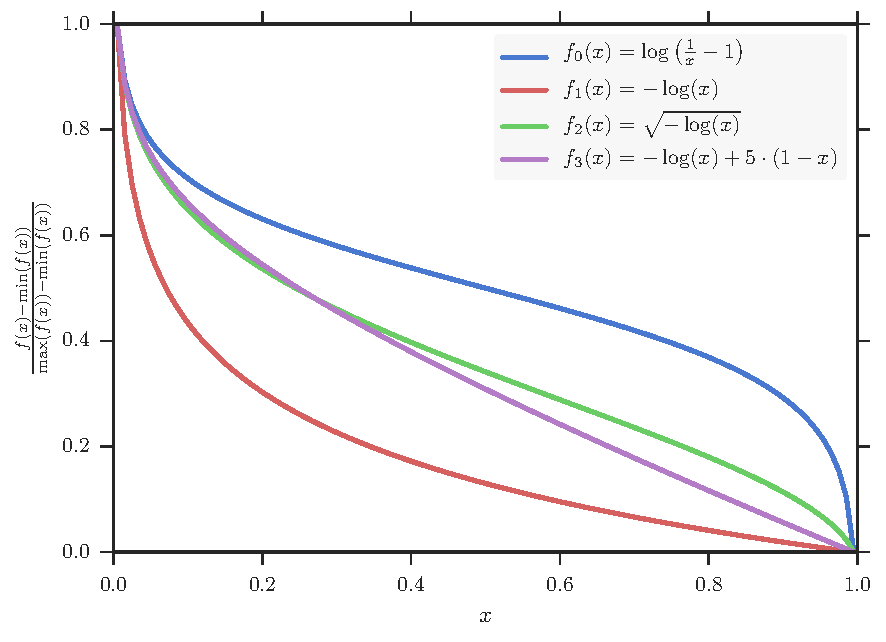
\includegraphics[width=0.7\textwidth]{images/xtransform.pdf}
	\caption{The transformations applied to the $x$ distribution, normalized to the range $[0,1]$.}
	\label{fig:xtransform}
\end{figure}
%
All transformations increase the point density in the low $x$ region, where most events should fall into.
Compared against $f_1$, the other functions also accomplish a higher point density in the high $x$ region.
Some observables in specific processes might benefit from this.

We can look at the actual $x$ distribution in the process considered in this thesis.
In \figref{fig:x_compare} it is plotted for one of the gluons involved in the process $gg \rightarrow H + j$ at leading order for a center-of-mass energy of $\sqrt{s} = \SI{13}{\tera\electronvolt}$.
For comparison, the respective distribution for the functions $f_0$ to $f_3$ is also shown.
In the bare distribution, the number of events per bin increases rapidly towards low $x$.
It is obvious that the reproduction of the low $x$ region is poor for this linear binning.
We expect that for some $x>0$ the number of events approaches zero, because there has to be at least enough momentum transfer to produce the Higgs boson and the jet.
To see this with linear binning, one would need a huge amount of bins.
In contrast, the transformations are able to project the low $x$ peak to a higher number of bins than the naive linear binning.
Additionally, they all approach zero for a finite value (note that high values of $f(x)$ correspond to low values of $x$).
Due to the normalization, this happens at $1$.
For all transformed distributions, it should be possible to interpolate them with a reasonable number of sampling points.
The function $f_1(x)$ looks most promising, as it allocates many bins for the peak region, which should be the most relevant for this process.

%
\begin{figure}[]
	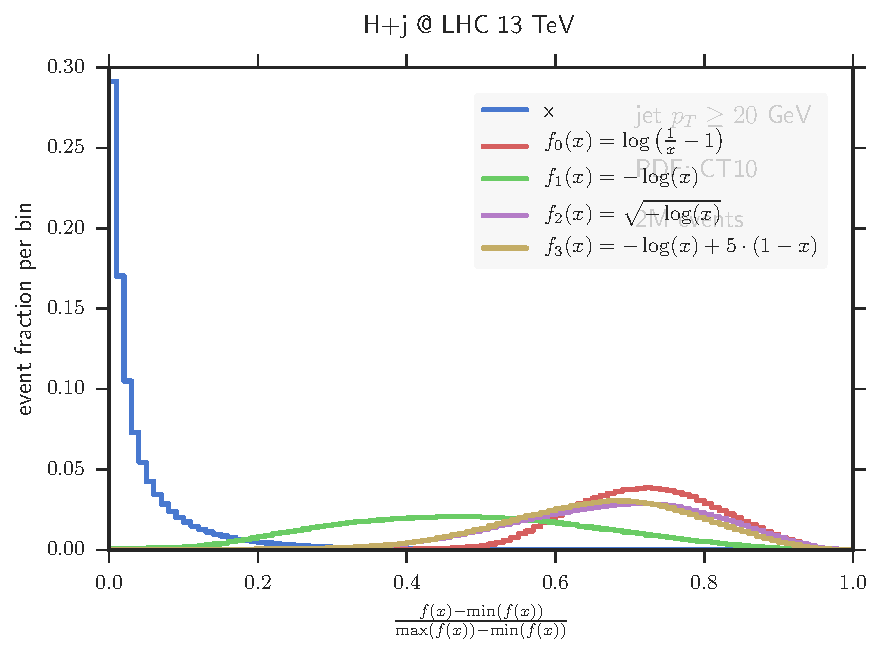
\includegraphics[width=0.7\textwidth]{images/x_compare.pdf}
	\caption{The event fraction per bin for the different transformations.}
	\label{fig:x_compare}
\end{figure}
%

If we want to be more specific, we can extract the dependence of the observables on $x$ and $f(x)$, respectively, from the generated events.
This is shown in \figref{fig:hpt_compare} for the transverse momentum $p_\perp$ and in \figref{fig:hy_compare} for the rapidity $y$ of the Higgs boson.
We see that the rapidity heavily depends on low $x$ values.
One half of the contributions comes from values $x \leq \num{0.03}$.
Values above \num{0.3} are in practice negligible.
The transformations reveal a substructure of the peak that is impossible to see with the linear binning.
Compared to the rapidity, the transverse momentum has a higher percentage of high $x$ values.
Nevertheless, it is still dominated by the low $x$ region.

For both observables all considered functions are a reasonable choice.
Especially for the rapidity, the function $f_1(x)$ seems to be best suited.
Hence, it will be the transformation used in all following grid calculations.
%
\begin{figure}[]
	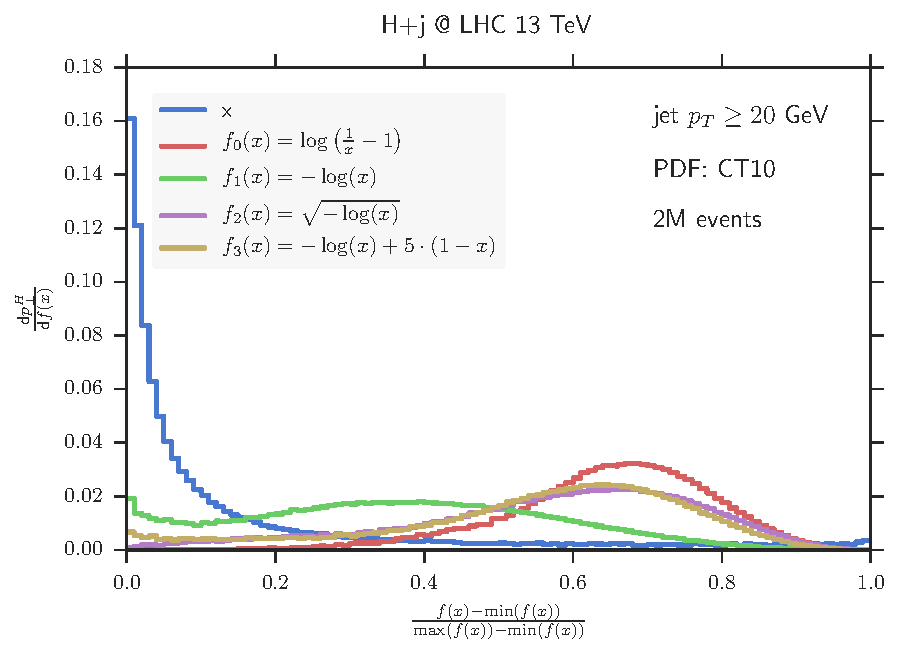
\includegraphics[width=0.7\textwidth]{images/hpt_compare.pdf}
	\caption{The transverse momentum $p_\perp$ of the Higgs boson differential in f(x).
				The ordinate shows the fraction per bin.}
	\label{fig:hpt_compare}
\end{figure}
%
\begin{figure}[]
	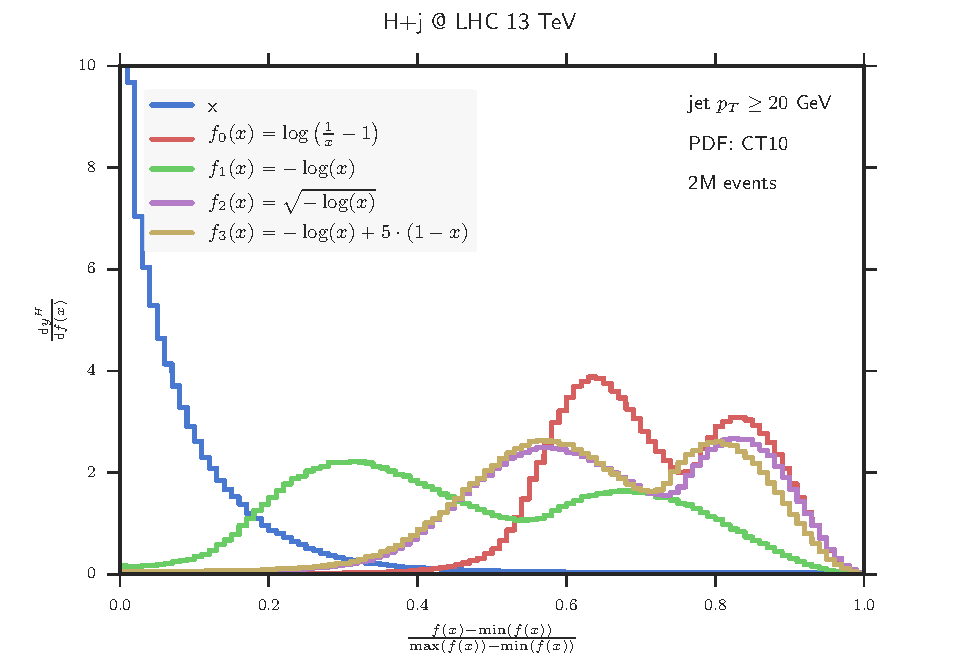
\includegraphics[width=0.7\textwidth]{images/hy_compare.pdf}
	\caption{The rapidity $y$ of the Higgs boson differential in f(x).
				The ordinate shows the fraction per bin.}
	\label{fig:hy_compare}
\end{figure}
%
\section{Interpolation accuracy}
In this section we will prove, that the grids are able to reproduce the reference distributions up to the available interpolation accuracy.
For each observable, one high precision grid and one lower precision grid is used.
In the 0- and 1-jet cases, the high precision grid has \num{50} bins in $x$ and the lower precision grid has \num{30} bins in $x$.
In the 2-jet case, the high precision grid has \num{70} bins and the lower precision one has \num{50} bins.
This is because with higher jet multiplicity, the influence of high $x$ values increases while in all cases the same transformation is used to smooth the distribution.
As we have seen in \cref{sec:xtransform}, this transformation favors low values of $x$, so a relatively high number of grid points is needed to accurately represent the high $x$ region.
For all the following calculations, the scale parameters have been fixed to the mass of the Higgs boson.
Therefore, $Q^2$ does not change and only one bin is used.
To achieve better comparability, \appl{} is configured to use fourth order interpolation, which is the same as is hardcoded into the \fnlo{} library.
A sample of \num{10} million events is used to fill the grids.

\Cref{fig:hnlo_validation} shows the ratio of the results obtained by convoluting the grids with the CT10 PDF to the reference distributions for the 0-jet process.
Using the high precision grid, all errors are below \SI{0.1}{\percent}.
\appl{} and \fnlo{} show roughly the same accuracy.
The effect of using a smaller grid is considerably bigger for the $p_\perp$ distributions than for the rapidity distributions.
This can be understood by looking back at \cref{fig:hpt_compare,fig:hy_compare} in \cref{sec:xtransform}.
There we saw, that high values of $x$ are completely negligible for the rapidity distribution and that it can be interpolated very well by using a logarithmic transformation.
The $p_\perp$ distribution is still dominated by small values of $x$, but compared to the rapidity large $x$-values have a bigger influence.
Thereby, the interpolation is not as optimal.
Here, the smaller grid also has a more severe impact on the \appl{} result than on the \fnlo{} one.

With one jet (\cref{fig:hjnlo_validation}), the errors in the reproduction of the $p_\perp$ become notably larger.
Even with the high precision grid, \fnlo{} produces errors for individual bins of the $p_\perp$ distributions, that are large compared to the other bins.
The errors of the largest outliers are about \SI{2}{\percent}.
In comparison, the errors produced by \appl{} with the high precision grid are of the order of \SI{0.01}{\percent}.
The main difference between the two packages that remains in the used configuration is the interpolation function.
Both use a kind of Lagrangian polynomials, but the implementations differ.
It might be possible, that the function used by \appl{} is more appropriate in this case.
Nonetheless, the reproduction of the rapidity distributions is still very good with all grids.
This is because the rapidity is not much influenced by additional jets.

The case of two jets is shown in \cref{fig:hjjnlo_validation}.
Here the grids with \num{50} bins produce relatively large errors.
With the high precision grid, however, \appl{} still allows a very good reproduction.
\fnlo{}, by contrast, features large outliers with errors of several percent.
This can be attributed to the statistics.
\Cref{fig:hpt_100m} proves that the reproduction is much better with a 100 million event sample, albeit still being worse than with \appl{}.
The problem with the $H + 2j$ process is that the event generator produces many negative weights, so that high statistics is needed to obtain a smooth distribution.
For some reason, this affects \fnlo{} more than \appl{}.
%
\begin{sidewaysfigure}
\centering
\begin{subfigure}[]{0.49\textwidth}
	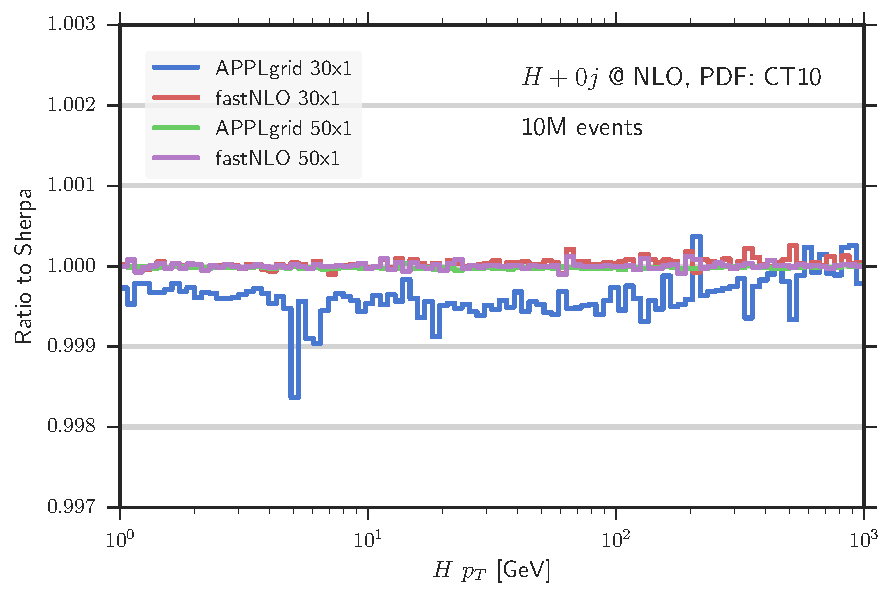
\includegraphics[width=\textwidth]{images/hnlo_hpt_50v30.pdf}
\end{subfigure}
\hfill
\begin{subfigure}[]{0.49\textwidth}
	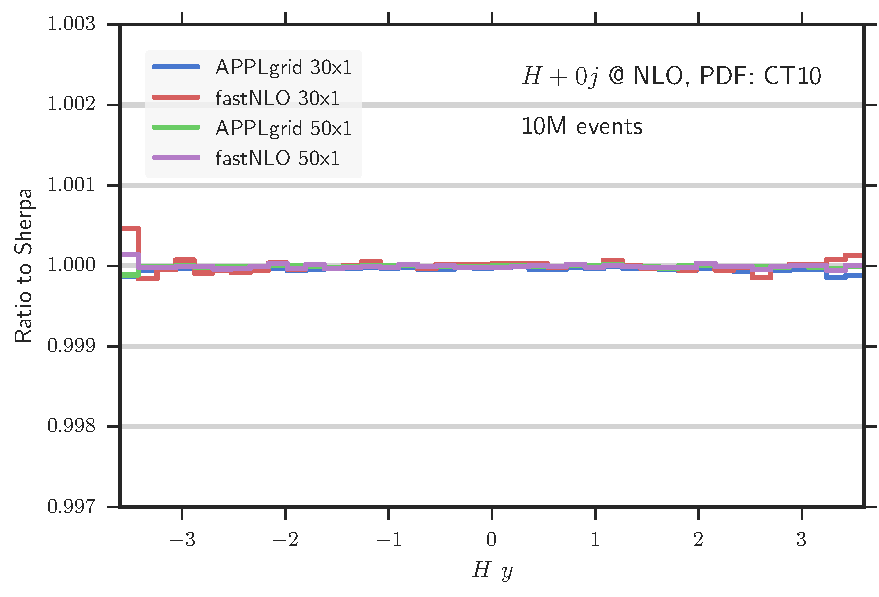
\includegraphics[width=\textwidth]{images/hnlo_hy_50v30.pdf}
\end{subfigure}

\begin{subfigure}[]{0.49\textwidth}
	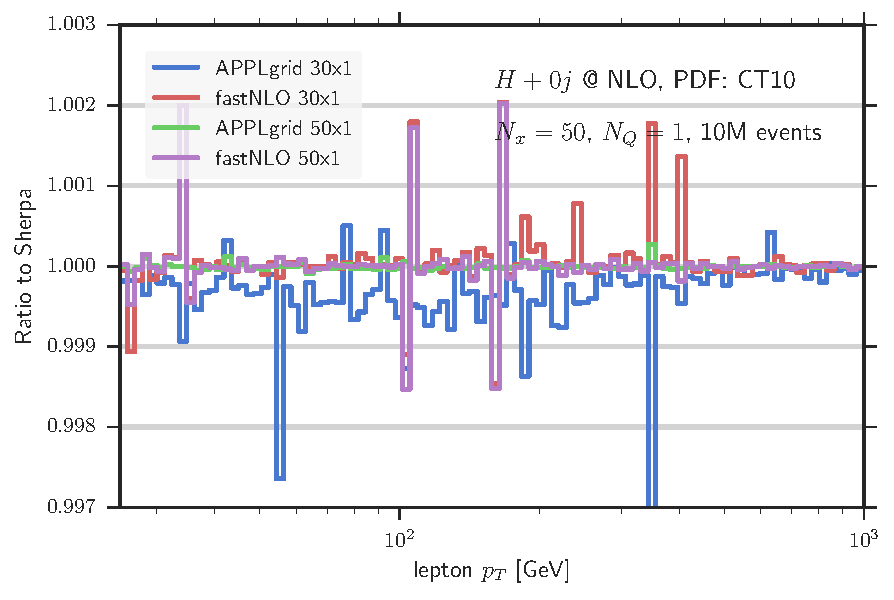
\includegraphics[width=\textwidth]{images/hnlo_lpt_50v30.pdf}
\end{subfigure}
\hfill
\begin{subfigure}[]{0.49\textwidth}
	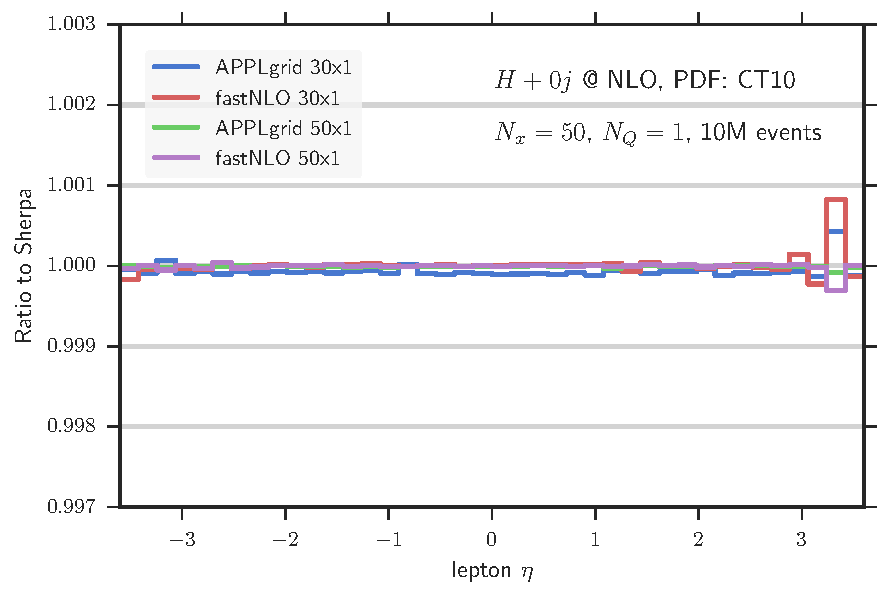
\includegraphics[width=\textwidth]{images/hnlo_leta_50v30.pdf}
\end{subfigure}
\caption{H+0j NLO}
\label{fig:hnlo_validation}
\end{sidewaysfigure}
%
\begin{sidewaysfigure}
\centering
\begin{subfigure}[]{0.49\textwidth}
	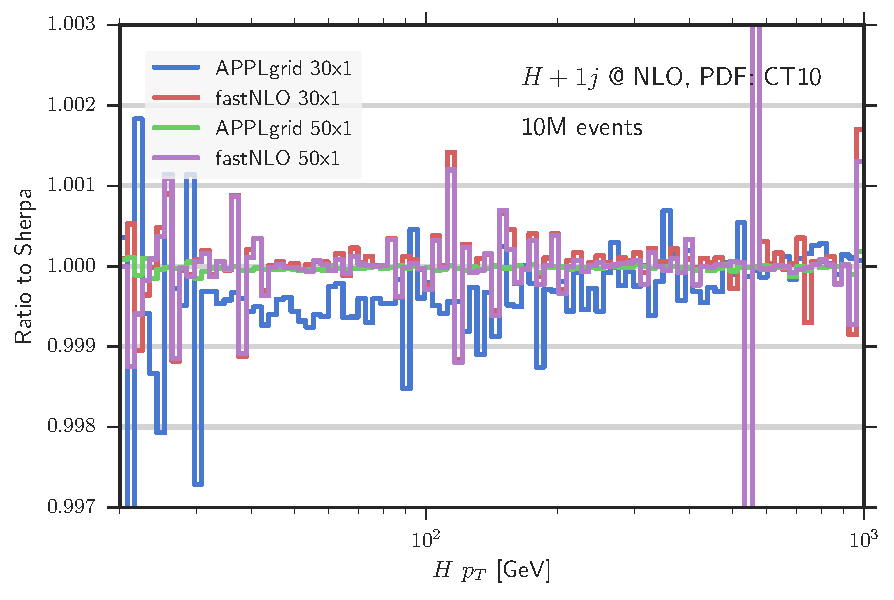
\includegraphics[width=\textwidth]{images/hjnlo_hpt_50v30.pdf}
\end{subfigure}
\hfill
\begin{subfigure}[]{0.49\textwidth}
	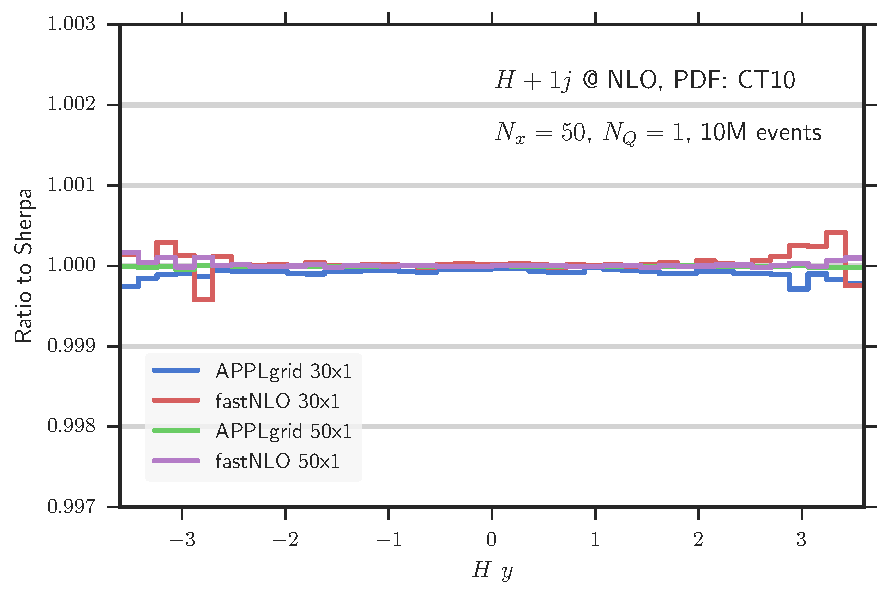
\includegraphics[width=\textwidth]{images/hjnlo_hy_50v30.pdf}
\end{subfigure}

\begin{subfigure}[]{0.49\textwidth}
	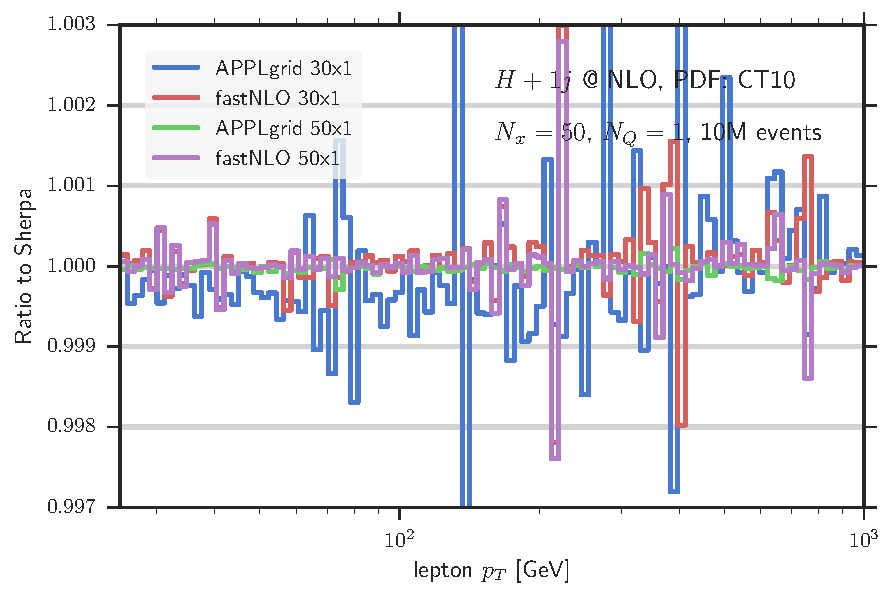
\includegraphics[width=\textwidth]{images/hjnlo_lpt_50v30.pdf}
\end{subfigure}
\hfill
\begin{subfigure}[]{0.49\textwidth}
	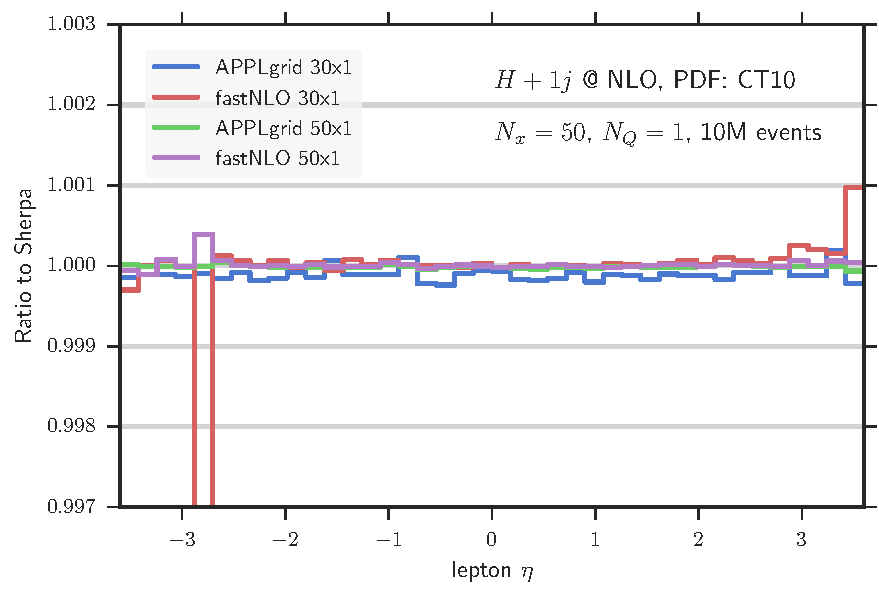
\includegraphics[width=\textwidth]{images/hjnlo_leta_50v30.pdf}
\end{subfigure}
\caption{H+1j NLO}
\label{fig:hjnlo_validation}
\end{sidewaysfigure}
%
\begin{sidewaysfigure}
\centering
\begin{subfigure}[]{0.49\textwidth}
	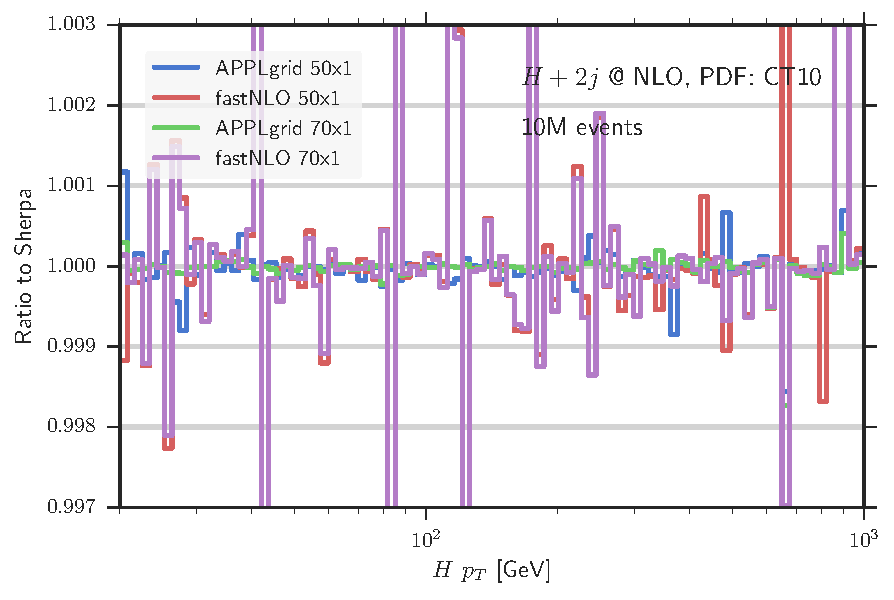
\includegraphics[width=\textwidth]{images/hjjnlo_hpt_70v50.pdf}
\end{subfigure}
\hfill
\begin{subfigure}[]{0.49\textwidth}
	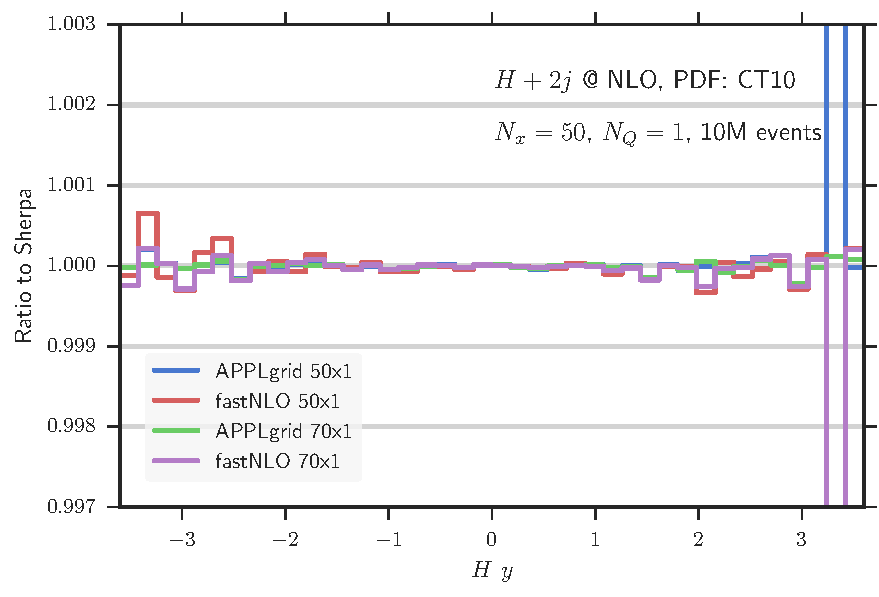
\includegraphics[width=\textwidth]{images/hjjnlo_hy_70v50.pdf}
\end{subfigure}

\begin{subfigure}[]{0.49\textwidth}
	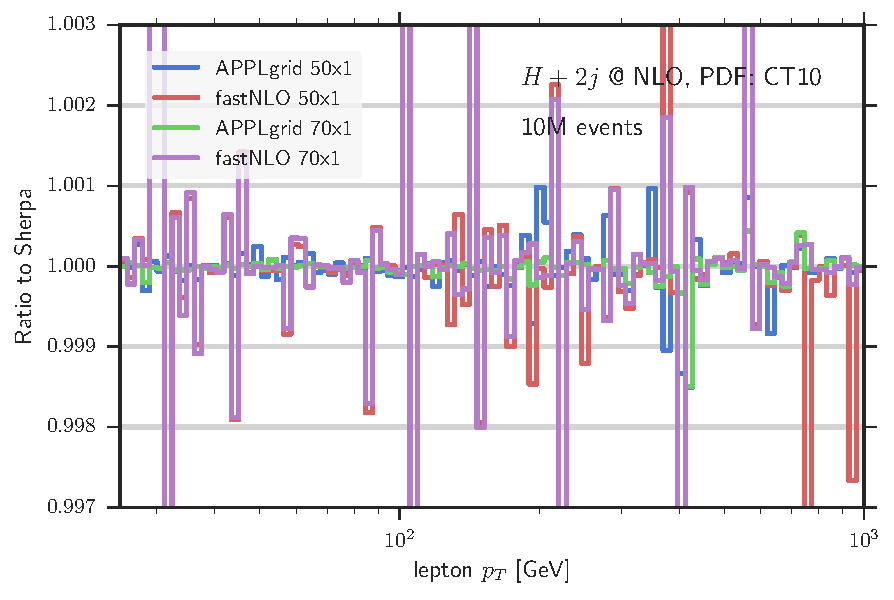
\includegraphics[width=\textwidth]{images/hjjnlo_lpt_70v50.pdf}
\end{subfigure}
\hfill
\begin{subfigure}[]{0.49\textwidth}
	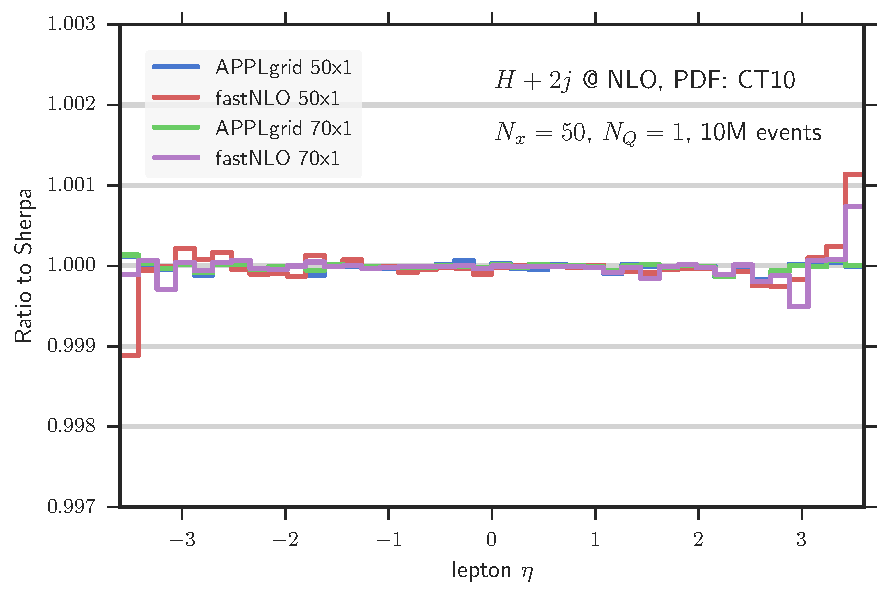
\includegraphics[width=\textwidth]{images/hjjnlo_leta_70v50.pdf}
\end{subfigure}
\caption{H+2j NLO}
\label{fig:hjjnlo_validation}
\end{sidewaysfigure}
%
\begin{figure}
	\centering
	\begin{subfigure}[]{0.49\textwidth}
		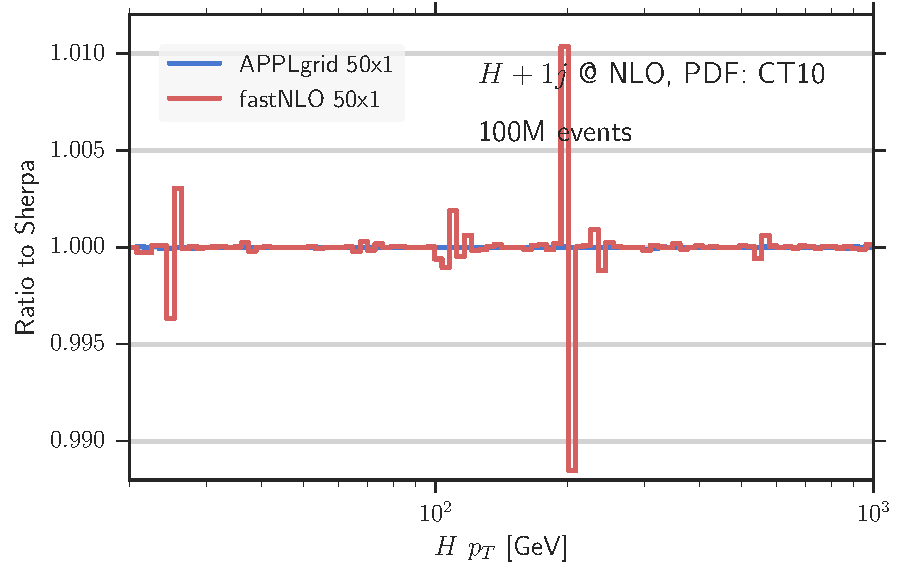
\includegraphics[width=\textwidth]{images/hjnlo_hpt_100m.pdf}
		\caption{$H + 1j$}
	\end{subfigure}
	\hfill
	\begin{subfigure}[]{0.49\textwidth}
		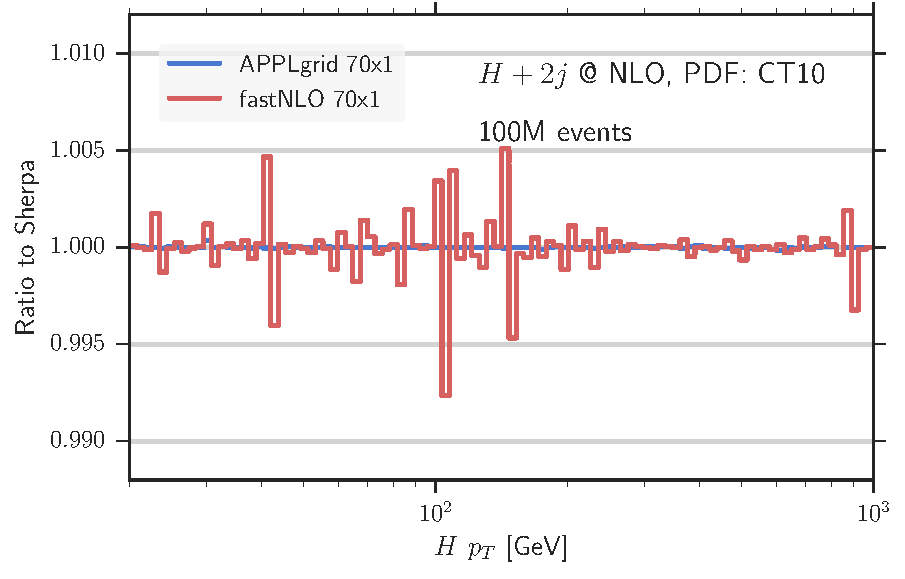
\includegraphics[width=\textwidth]{images/hjjnlo_hpt_100m.pdf}
		\caption{$H + 2j$}
	\end{subfigure}
	\caption{The effect of higher statistics on the interpolation.
				With two jets the 100 million event sample gives notably better results than the 10 million event sample in \cref{fig:hjjnlo_validation}.
				With one jet the errors are roughly the same.}
	\label{fig:hpt_100m}
\end{figure}
%
\section{Parameter variation}
\subsection{Scale factor variation}
Now that we have verified that the grids produced by \appl{} and \fnlo{} are able to reproduce the reference distributions up to the interpoation accuracy, we can take a look at the variation of the QCD parameters.
In this section we will examine the results obtained by varying the renormalization and factorization scales.
\appl{} and \fnlo{} both have methods implemented that allow to change the scales when calculating NLO cross sections.
There are different approaches to this.
The original method used by \appl{} is to apply the renormalization group equation for the renormalization scale and calculate the LO DGLAP splitting functions using \hoppet{} \cite{hoppet} to vary the factorization scale.
\fnlo{} originally did not allow the use of \hoppet{} and instead stored individual grids for each desired factorization scale.
This approach is not as flexible and leads to larger grid files but the calculation of the cross section is much faster.
However, since version 2.3 \fnlo{} can also be used in combination with \hoppet{}.
Another method, called \enquote{flexible-scale table}, is also implemented in \fnlo{}.
It stores fully scale-independent weights and allows for arbitrary and independent variation of the scale factors without the need of splitting functions.
As this feature is not yet implemented in \mcgrid{} (but will be in a future release), the first method is used in the following calculations.

The reference histograms are again generated with Sherpa using the CT10 PDF.
One central scale $\mu_R = \mu_F = m_H$ and two additional scales $2 \mu$ and $\frac{1}{2} \mu$ are used.
During the central scale run, grids for the transverse momentum of the Higgs boson are filled by \appl{} and \fnlo{} using an \mcgrid{}-enabled \rivet{} analysis.
This is done for Higgs production with zero and one jets using an event sample of 100 million events in each case.
In \cref{fig:scalesvar_hnlo_appl,fig:scalesvar_hnlo_fnlo} the reference distributions are compared to the results from \appl{} and \fnlo{} in the 0-jet case.
We observe a strong scale dependence, indicating that higher order terms entail large corrections.
This turns out to be true \cite{gfusionnnlo1,gfusionnnlo2}.
It can be seen, that the accuracy of the reproduction is very good in both cases.
The discrepancies at low $p_\perp$ in \cref{fig:scalesvar_hnlo_appl} are due to an insufficient phasespace run (the first ten million events have been used), meaning that during the fill run $x$-values emerged that were not expected by \appl{}.
The \fnlo{} grid was prepared with the same phasespace run and obviously it responds to these events in a different way resulting in a precise reproduction throughout the range of considered values.
Using a larger phasespace run, the inaccuracies with \appl{} would of course vanish.
%
\begin{figure}
	\centering
	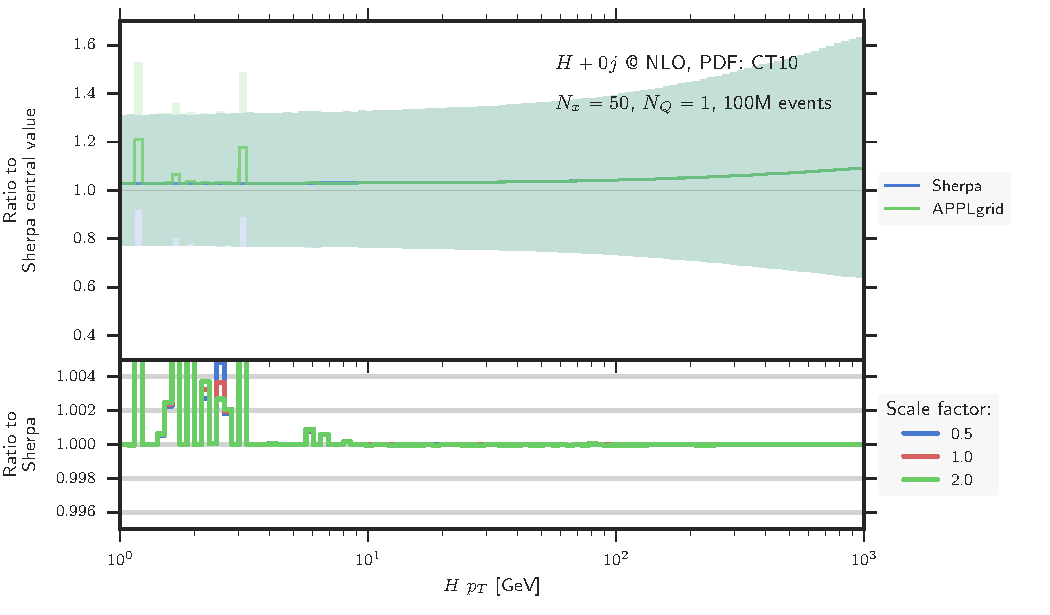
\includegraphics[width=\textwidth]{images/scalesvar_hnlo_appl.pdf}
	\caption{Scale variation appl}
	\label{fig:scalesvar_hnlo_appl}
\end{figure}
%
\begin{figure}
	\centering
	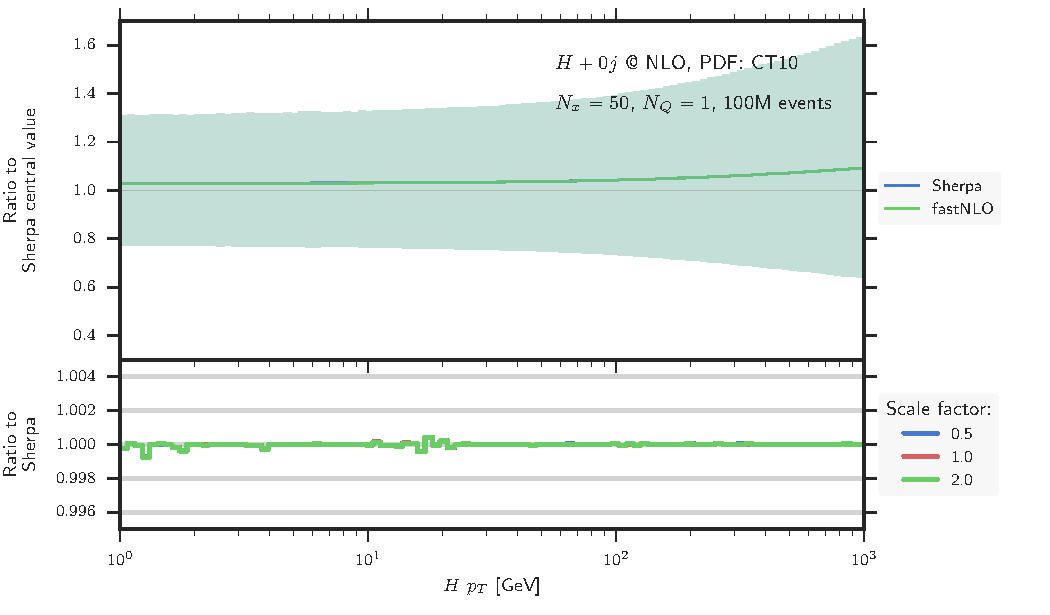
\includegraphics[width=\textwidth]{images/scalesvar_hnlo_fnlo.pdf}
	\caption{Scale variation fnlo}
	\label{fig:scalesvar_hnlo_fnlo}
\end{figure}
%

In the 1-jet case, shown in \cref{fig:scalesvar_hjnlo_appl,fig:scalesvar_hjnlo_fnlo}, the scale dependence is more complicated.
Still, \appl{} is able to reproduce all three scales at the permille level.
\fnlo{}, on the contrary, shows an unexpected behaviour.
There are systematic deviations that increase towards high transverse momenta.
As the error is definitely not caused by statistical fluctuations and because the central scale is reproduced very well, there is probably a mistake in the implementation of the evolution.
A similar behaviour can be observed with \appl{} as well, when the 2-jet case is considered.
Therefore, this does not seem to be a problem of \fnlo{} alone.
This problem is object of further investigations.
%
\begin{figure}
	\centering
	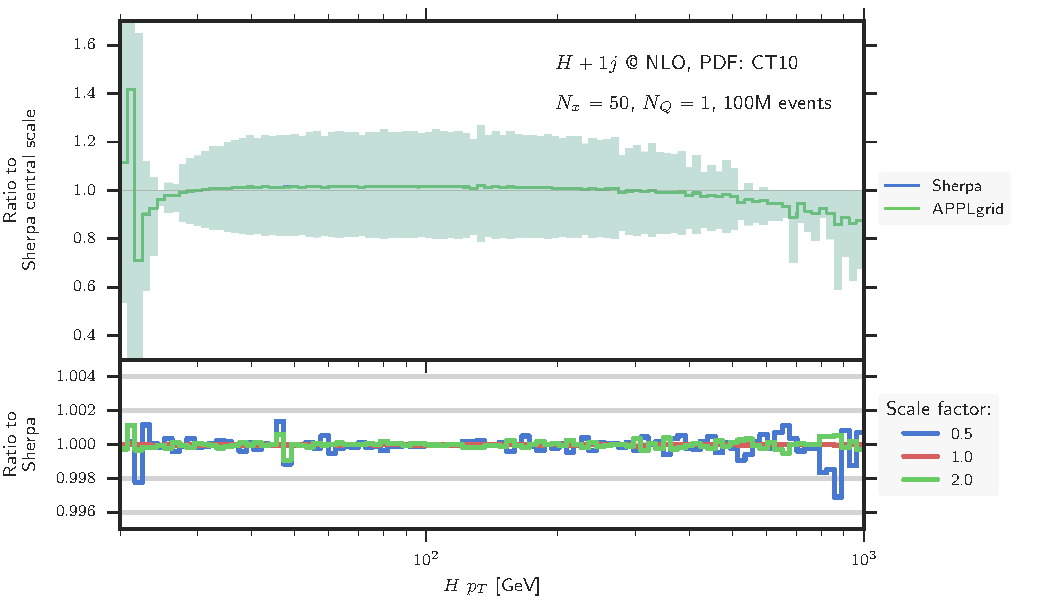
\includegraphics[width=\textwidth]{images/scalesvar_hjnlo_appl.pdf}
	\caption{Scale variation appl}
	\label{fig:scalesvar_hjnlo_appl}
\end{figure}
%
\begin{figure}
	\centering
	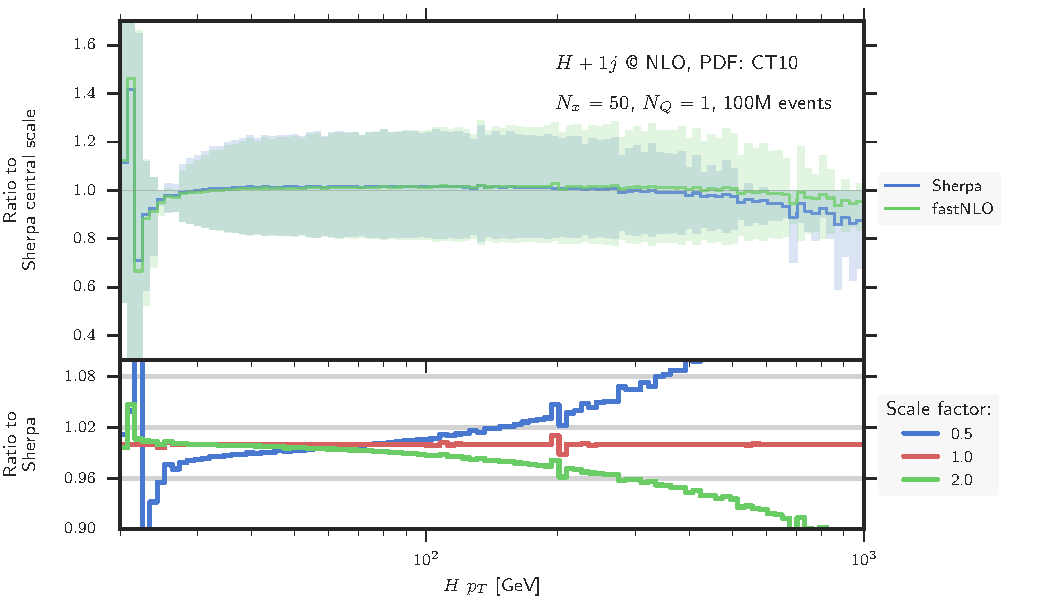
\includegraphics[width=\textwidth]{images/scalesvar_hjnlo_fnlo.pdf}
	\caption{Scale variation fnlo}
	\label{fig:scalesvar_hjnlo_fnlo}
\end{figure}
%
\subsection{Reweighting to a different PDF}
In addition to the variation of the scale factors, it is possible to change the PDF as well.
As an example, the transverse momentum of the Higgs boson is considered again.
Grids that have been filled with the CT10 PDF are convoluted with the central value of the NNPDF3.0 set \textit{a posteriori}.
They are compared to the reference distribution, that has been produced by \sherpa{} using NNPDF3.0 explicitly, at three different scales.
The results are shown in \cref{fig:pdfvar_hnlo_appl,fig:pdfvar_hnlo_fnlo} for \appl{} and \fnlo{}, respectively.
Again, we observe a very good reproduction.
The magnitude of the errors is similar to the results of the previous section (cf. \cref{fig:scalesvar_hnlo_appl,fig:scalesvar_hnlo_fnlo}).
As has already been explained above, the discrepancies in the \appl{} plot at low $p_\perp$ originate from an insufficient phasespace run that did not cover the whole $x$-range.
They do not indicate any problems with the interpolation (which is proven by the \fnlo{} result in \cref{fig:pdfvar_hnlo_fnlo}) and are fixable.
%
\begin{figure}
	\centering
	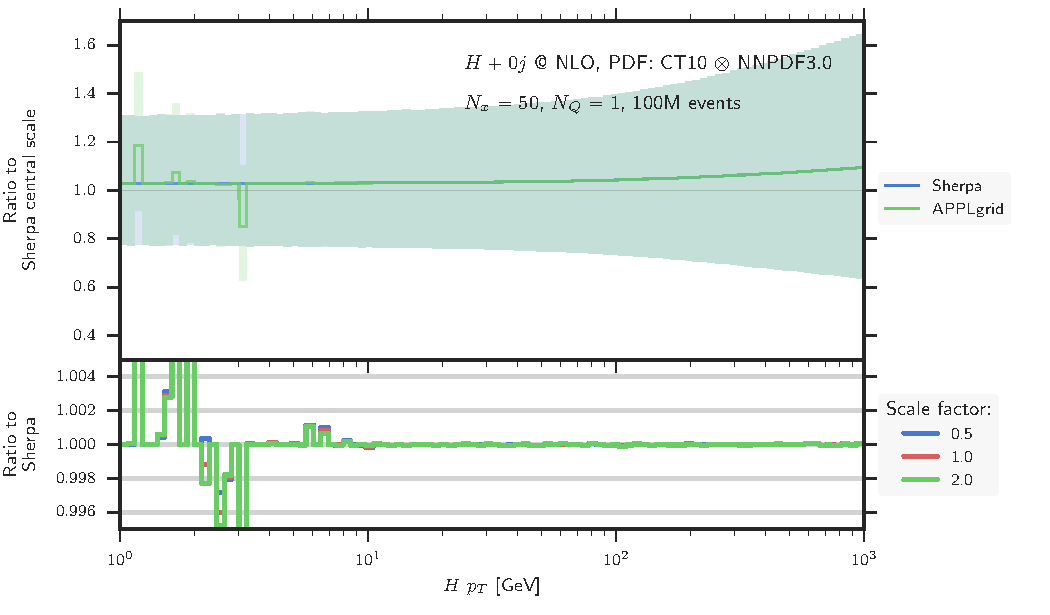
\includegraphics[width=\textwidth]{images/pdfvar_hnlo_appl.pdf}
	\caption{PDF variation appl}
	\label{fig:pdfvar_hnlo_appl}
\end{figure}
%
\begin{figure}
	\centering
	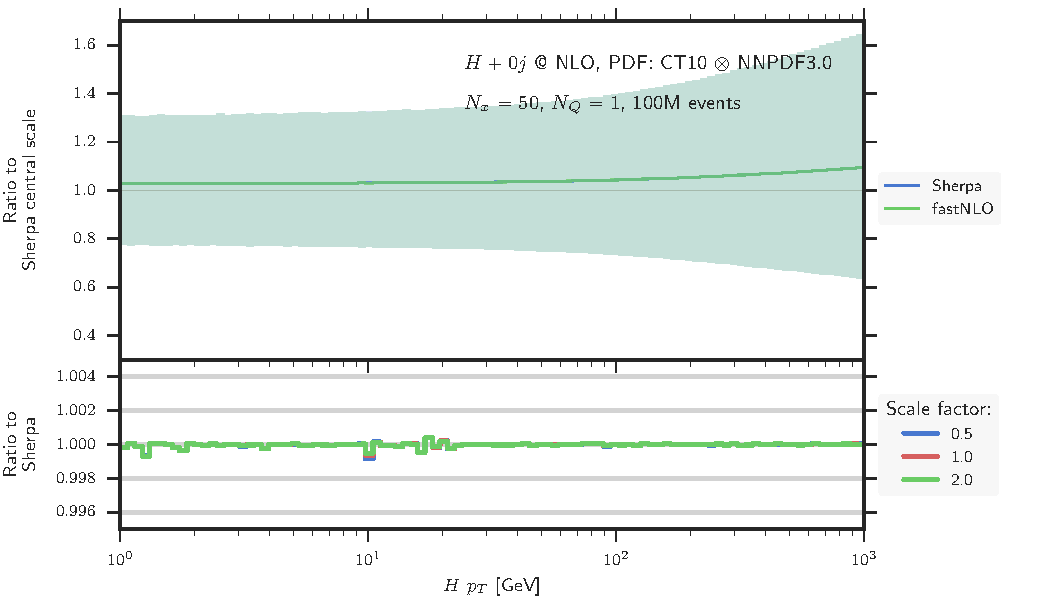
\includegraphics[width=\textwidth]{images/pdfvar_hnlo_fnlo.pdf}
	\caption{PDF variation fnlo}
	\label{fig:pdfvar_hnlo_fnlo}
\end{figure}
%
